\documentclass{article}
\usepackage[utf8]{inputenc}
\usepackage{authblk}
\usepackage{setspace}
\usepackage[margin=1.25in]{geometry}
\usepackage{graphicx}
\usepackage{xcolor}
\usepackage{float}
\graphicspath{ {./figures/} }
\usepackage{amsmath,amssymb,amsfonts}
\usepackage{booktabs}
\usepackage{natbib}
\usepackage{hyperref}
\hypersetup{colorlinks=true, linkcolor=blue, citecolor=blue, urlcolor=blue}

\title{\textbf{Federal Reserve Announcement Days and US Equity Volatility: An Event Study of FOMC Statements, 2016--2026}}
\author[1]{SIQuant Research}
\affil[1]{Hypothesis $\times$ Quant}
\date{\today}
\onehalfspacing

\begin{document}
\maketitle

\begin{abstract}
\noindent \textbf{Hypothesis:} $H_0$: mean $|$return$|$ of the S\&P 500 on FOMC announcement days equals that of ordinary sessions; $H_1$: it is larger \\
\textbf{Data:} 81 FOMC statements (88 listed) matched to S\&P 500 and VIX closes, 2016-11-02 to 2026-09-16 \\
\textbf{Method:} 10,000-draw placebo over ordinary sessions (meeting $\pm1$ day excluded); Bonferroni $\alpha=0.025$ for two outcomes \\
\textbf{Results:} Mean $|$return$|$ 0.846\% versus placebo 0.724\% (one-sided $p=0.1021$); mean $\Delta$VIX 0.64\% versus placebo 0.36\% ($p=0.6275$ for a larger fall).  \\
\textbf{Research decision:} \colorbox[rgb]{0.75,0.15,0.15}{\textcolor{white}{\textbf{\,REJECTED\,}}}
\end{abstract}

\section{Design}
FOMC statements are released at 14:00 US/Eastern, two hours before the cash close, so the close-to-close return of the release date contains the full announcement reaction together with 5.5 hours of pre-announcement trading, which dilutes the measured effect. The placebo draws ordinary sessions from the same sample, so volatility regimes are matched on average \citep{lucca2015premium}.

\section{Results}
\begin{table}[H]
\centering
\caption{S\&P 500 and VIX on FOMC announcement days by policy action}
\begin{tabular}{lcccc}
\toprule
Action & Events & Mean $|$return$|$ & Mean return & Mean $\Delta$VIX \\
\midrule
HOLD & 51 & 0.73\% & 0.03\% & 0.14\% \\
HIKE & 20 & 1.11\% & 0.01\% & -1.73\% \\
CUT & 10 & 0.90\% & -0.55\% & 7.91\% \\
\bottomrule
\end{tabular}
\end{table}


\begin{figure}[H]
\centering
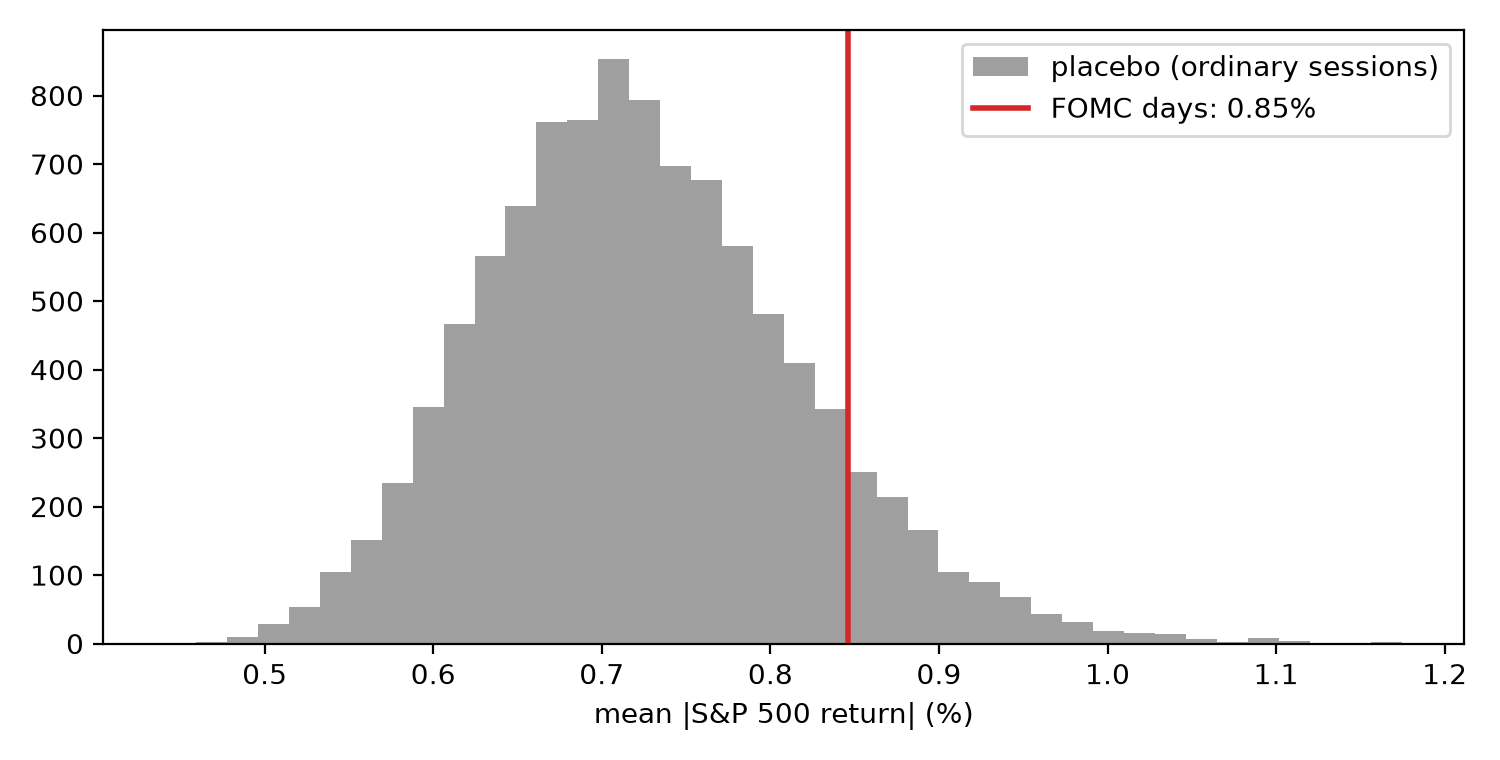
\includegraphics[width=0.8\textwidth]{fig1_fomc_abs_return_placebo.png}
\caption{Mean absolute S\&P 500 return on FOMC days against the placebo distribution.}
\end{figure}

The signed mean return on FOMC days is -0.048\% (t=-0.36).

\section{Limitations}
The sample is short (about ten years, one tightening cycle) and clustered in 2020 when unscheduled meetings coincided with the COVID shock; a regime-matched placebo is left to follow-up work. Intraday data would isolate the announcement window but are not free.


\bibliographystyle{plainnat}
\bibliography{references}

\end{document}
